\documentclass{article}
\usepackage{tikz}
\usetikzlibrary{knots}

\newcommand{\KP}[1]{%
  \begin{tikzpicture}[baseline=-\dimexpr\fontdimen22\textfont2\relax,yscale=-1,xscale=1]
  #1
  \end{tikzpicture}%
}


\begin{document}

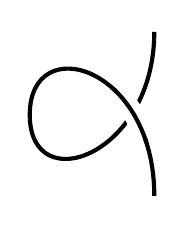
\begin{tikzpicture}[x=0.75pt,y=0.75pt,yscale=-1,xscale=1]
  \begin{knot}[
    consider self intersections,
    clip width=5,
  ]
    \strand [line width=1.5]    (129.51,238.92) .. controls (129.51,175.92) and (69.51,158.92) .. (69.51,199.92) .. controls (69.51,240.92) and (129.51,219.92) .. (129.51,159.92) ;
  \end{knot}
\end{tikzpicture}

\newcommand{\KPA}[0]{%
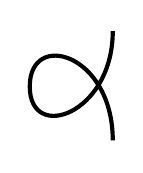
\begin{tikzpicture}[baseline=-103pt,x=0.5pt,y=0.5pt,yscale=-1,xscale=1]
  \begin{knot}[
    consider self intersections,
    clip width=5,
  ]
    \strand [line width=1.5]    (129.51,238.92) .. controls (129.51,175.92) and (69.51,158.92) .. (69.51,199.92) .. controls (69.51,240.92) and (129.51,219.92) .. (129.51,159.92) ;
  \end{knot}
\end{tikzpicture}%
}


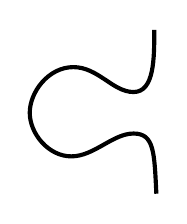
\begin{tikzpicture}[x=0.75pt,y=0.75pt,yscale=-1,xscale=1]
  \begin{knot}[
    consider self intersections,
    clip width=5,
  ]
    \strand [line width=1.5] (230.51,238.92) .. controls (229.51,218.92) and (229.51,209.92) .. (219.51,209.92) .. controls (209.51,209.92) and (200.51,220.92) .. (189.51,220.92) .. controls (178.51,220.92) and (169.51,209.92) .. (169.51,199.92) .. controls (169.51,189.92) and (178.51,177.92) .. (190.51,177.92) .. controls (202.51,177.92) and (209.51,189.92) .. (219.51,189.92) .. controls (229.51,189.92) and (229.51,173.92) .. (229.51,159.92) ;
  \end{knot}
\end{tikzpicture}

\newcommand{\KPB}[0]{%
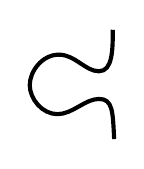
\begin{tikzpicture}[baseline=-103pt,x=0.5pt,y=0.5pt,yscale=-1,xscale=1]
  \begin{knot}[
    consider self intersections,
    clip width=5,
  ]
    \strand [line width=1.5] (230.51,238.92) .. controls (229.51,218.92) and (229.51,209.92) .. (219.51,209.92) .. controls (209.51,209.92) and (200.51,220.92) .. (189.51,220.92) .. controls (178.51,220.92) and (169.51,209.92) .. (169.51,199.92) .. controls (169.51,189.92) and (178.51,177.92) .. (190.51,177.92) .. controls (202.51,177.92) and (209.51,189.92) .. (219.51,189.92) .. controls (229.51,189.92) and (229.51,173.92) .. (229.51,159.92) ;
\end{knot}
\end{tikzpicture}%
}

$$
\left\langle \KPA \right\rangle 
= A \left\langle \KPA \right\rangle
+ B \left\langle \KPB \right\rangle
$$

\end{document}